\documentclass[a4paper]{arrowhead}

\usepackage[yyyymmdd]{datetime}
\usepackage{etoolbox}
\usepackage[utf8]{inputenc}
\usepackage{multirow}
\usepackage{hyperref}

\renewcommand{\dateseparator}{-}

\setlength{\parskip}{1em}

%% Special references
\newcommand{\fref}[1]{{\textcolor{ArrowheadBlue}{\hyperref[sec:functions:#1]{#1}}}}
\newcommand{\mref}[1]{{\textcolor{ArrowheadPurple}{\hyperref[sec:model:#1]{#1}}}}
\newcommand{\pdef}[1]{{\textcolor{ArrowheadGrey}{#1\label{sec:model:primitives:#1}\label{sec:model:primitives:#1s}\label{sec:model:primitives:#1es}}}}
\newcommand{\pref}[1]{{\textcolor{ArrowheadGrey}{\hyperref[sec:model:primitives:#1]{#1}}}}

\newrobustcmd\fsubsection[3]{
  \addtocounter{subsection}{1}
  \addcontentsline{toc}{subsection}{\protect\numberline{\thesubsection}function \textcolor{ArrowheadBlue}{#1}}
  \renewcommand*{\do}[1]{\rref{##1},\ }
  \subsection*{
    \thesubsection\quad
    operation
    \textcolor{ArrowheadBlue}{#1}
    (\notblank{#2}{\mref{#2}}{})
    \notblank{#3}{: \mref{#3}}{}
  }
  \label{sec:functions:#1}
}
\newrobustcmd\msubsection[2]{
  \addtocounter{subsection}{1}
  \addcontentsline{toc}{subsection}{\protect\numberline{\thesubsection}#1 \textcolor{ArrowheadPurple}{#2}}
  \subsection*{\thesubsection\quad#1 \textcolor{ArrowheadPurple}{#2}}
  \label{sec:model:#2} \label{sec:model:#2s} \label{sec:model:#2es}
}

\begin{document}

%% Arrowhead Document Properties
\ArrowheadTitle{Gateway Core System}
\ArrowheadType{System Description}
\ArrowheadTypeShort{SysD}
\ArrowheadVersion{4.6.0}
\ArrowheadDate{\today}
\ArrowheadAuthor{Rajmund Bocsi}
\ArrowheadStatus{RELEASE}
\ArrowheadContact{rbocsi@aitia.ai}
\ArrowheadFooter{\href{www.arrowhead.eu}{www.arrowhead.eu}}
\ArrowheadSetup
%%

%% Front Page
\begin{center}
  \vspace*{1cm}
  \huge{\arrowtitle}

  \vspace*{0.2cm}
  \LARGE{\arrowtype}
  \vspace*{1cm}

  %\Large{Service ID: \textit{"\arrowid"}}
  \vspace*{\fill}

  % Front Page Image
  %\includegraphics{figures/TODO}

  \vspace*{1cm}
  \vspace*{\fill}

  % Front Page Abstract
  \begin{abstract}
    This document provides system description for the \textbf{Gateway Core System}.
  \end{abstract}

  \vspace*{1cm}

%   \scriptsize
%   \begin{tabularx}{\textwidth}{l X}
%     \raisebox{-0.5\height}{
\includegraphics[width=2cm]{figures/artemis_logo}} & {ARTEMIS Innovation Pilot Project: Arrowhead\newline
%     THEME [SP1-JTI-ARTEMIS-2012-AIPP4 SP1-JTI-ARTEMIS-2012-AIPP6]\newline
%     [Production and Energy System Automation Intelligent-Built environment and urban infrastructure for sustainable and friendly cities]}
%   \end{tabularx}
%   \vspace*{-0.2cm}
 \end{center}

\newpage
%%

%% Table of Contents
\tableofcontents
\newpage
%%

\section{Overview}
\label{sec:overview}
\color{black}
This document describes the Gateway Core System, which exists to establish a secure connection between a consumer and a provider located in different clouds. The concept of the Gateway is described by figure \ref{fig:gateway_overview}. 

\begin{figure}[h!]
  \centering
  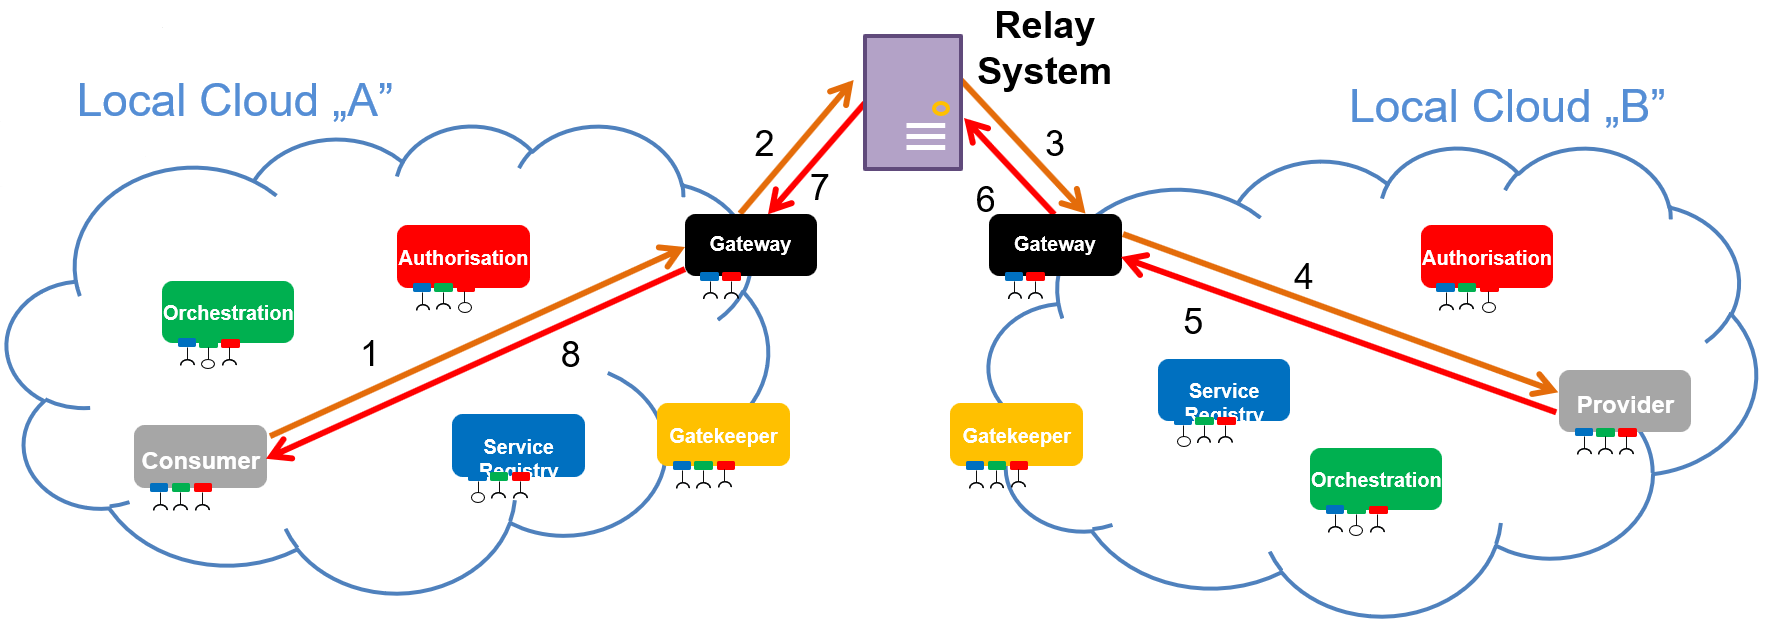
\includegraphics[width=16cm]{figures/gateway_overview.png}
  \caption{
    Overview of the Gateway Core System.
  }
  \label{fig:gateway_overview}
\end{figure}

The rest of this document is organized as follows.
In Section \ref{sec:prior_art}, we reference major prior art capabilities
of the system.
In Section \ref{sec:use}, we describe the intended usage of the system.
In Section \ref{sec:properties}, we describe fundamental properties
provided by the system.
In Section \ref{sec:delimitations}, we describe delimitations of capabilities
of the system.
In Section \ref{sec:services}, we describe the abstract service
operations produced by the system.
In Section \ref{sec:security}, we describe the security capabilities
of the system.

\subsection{Significant Prior Art}
\label{sec:prior_art}

The strong development on cloud technology and various requirements for digitisation and automation has led to the concept of Local Clouds (LC).

\textit{"The concept takes the view that specific geographically local automation tasks should be encapsulated and protected."} \cite{jerker2017localclouds}

Encapsulated and protected LCs means that when a consumer has to use a provider from an other cloud there is no easy way to do that. A gateway support system is needed to create a tunnel between the two application systems on which they can communicate each other without risking their cloud's security.  

\subsection{How This System Is Meant to Be Used}
\label{sec:use}

Gateway is a support core system of Eclipse Arrowhead LC and is responsible for providing secure communication channel between service consumers and providers that are in different clouds. 

The building of the secure channel is initiated by the two Gatekeeper Core Systems (one for each participating clouds) during the inter-cloud negotiation process. From an application system's point of view this happens automatically when a consumer can only find matching provider in an other cloud (and those clouds does not support direct access).

\subsection{System functionalities and properties}
\label{sec:properties}

\subsubsection {Functional properties of the system}
Gateway solves the following needs to fulfill the requirements of providing secure communication channels between clouds.

\begin{itemize}
    \item Enables the Gatekeeper core systems to establish a connection between the consumer and the provider through cloud boundaries.
    \item Enables the Gatekeeper core system to get its public key in order to ensure the connection security between the clouds.
    \item Enables the Workflow Choreographer core system to close unused gateway tunnels.
\end{itemize}

\subsubsection {Non functional properties of the system}
The Gateway implements certain authentication capabilities, meaning that Gateway makes decision whether a given system has right to use its services (i.e. only the Gatekeeper can initiate a gateway tunnel creation).

\subsubsection {Data stored by the system}
The Gateway Core System does not need any persistent storage.

\subsection{Important Delimitations}
\label{sec:delimitations}

The Gateway Core System can only run in secure mode.

Also, it needs at least one external relay application that is accessible from both participating clouds to enable the communication between application systems of the clouds. Furthermore, the Gatekeeper Core System is also needed to initiate the Gateway's tunnel creation operation.

\newpage

\section{Services produced}
\label{sec:services}

\msubsection{service}{echo}
The purpose of this service is to test the system availability. The service is offered for both application and core systems. 

\msubsection{service}{gw-public-key}
The purpose of this service is to provide the public key of the Gateway Core System. It is necessary to ensure the secure communication between the Gateways. 

\msubsection{service}{gw-connect-consumer}
The purpose of this service is to create an access point for the consumer to consume a specific service beyond the cloud boundaries. 

\msubsection{service}{gw-connect-provider}
The purpose of this service is to create a proxy that can consume a specific provider of the cloud in the name of a consumer beyond the cloud boundaries.

\msubsection{service}{gw-close-sessions}
The purpose of this service is to destroys the specified gateway tunnels and release their resources.

\newpage

\section{Security}
\label{sec:security}

The security of Eclipse Arrowhead - and therefore the security of Gateway - is relying on X.509 certificate trust chains. The Arrowhead trust chain consists of three level:
\begin{itemize}
    \item Master certificate: \texttt{arrowhead.eu}
    \item Cloud certificate: \texttt {my-cloud.my-company.arrowhead.eu}
    \item Client certificate: \texttt{my-client.my-cloud.my-company.arrowhead.eu}
\end{itemize}

For Arrowhead certificate profile see \url{https://github.com/eclipse-arrowhead/documentation}

\newpage

\bibliographystyle{IEEEtran}
\bibliography{bibliography}

\newpage

\section{Revision History}
\subsection{Amendments}

\noindent\begin{tabularx}{\textwidth}{| p{1cm} | p{3cm} | p{2cm} | X | p{4cm} |} \hline
\rowcolor{gray!33} No. & Date & Version & Subject of Amendments & Author \\ \hline

1 & YYYY-MM-DD & \arrowversion & & Xxx Yyy \\ \hline
\end{tabularx}

\subsection{Quality Assurance}

\noindent\begin{tabularx}{\textwidth}{| p{1cm} | p{3cm} | p{2cm} | X |} \hline
\rowcolor{gray!33} No. & Date & Version & Approved by \\ \hline

1 & YYYY-MM-DD & \arrowversion  &  \\ \hline

\end{tabularx}

\end{document}